\section{TINJAUAN PUSTAKA}

% Ubah konten-konten berikut sesuai dengan isi dari tinjauan pustaka
\subsection{Wajah}

% Contoh penggunaan referensi dari pustaka
% Newton pernah merumuskan \citep{Newton1687} bahwa \lipsum[8]
% Contoh penggunaan referensi dari persamaan
% Kemudian menjadi persamaan seperti pada persamaan \ref{eq:FirstLaw}.

Wajah merupakan bagian dari tubuh manusia yang menjadi fokus perhatian di dalam interaksi sosial, 
wajah memainkan peranan vital dengan menunjukan identitas dan emosi. Kemampuan manusia untuk mengetahui 
seseorang dari wajahnya sangat luar biasa. Kita dapat mengenali ribuan wajah karena frekuensi interaksi 
yang sangat sering ataupun hanya sekilas bahkan dalam rentang waktu yang sangat lama. Bahkan kita mampu 
mengenali seseorang walaupun terjadi perubahan pada orang tersebut karena bertambahnya usia atau 
pemakaian kacamata atau perubahan gaya rambut. Oleh karena itu wajah digunakan sebagai organ dari tubuh 
manusia yang dijadikan indikasi pengenalan seseorang. Dimana identitas, ekspresi, gender, umur dan etnik 
disebut dengan dalam wajah.

\subsection{Umur}
Umur merupakan rentang kehidupan yang diukur dengan tahun, dikatakan masa awal dewasa adalah usia 18 – 40 
tahun, dewasa madya adalah 41 – 60 tahun, dewasa lanjut lebih dari 60 tahun. Umur adalah lamanya hidup 
dalam tahun yang dihitung sejak dilahirkan\citep{MasaTubuh}.
% input gambar
\begin{figure} [H] \centering
    % Nama dari file gambar yang diinputkan
    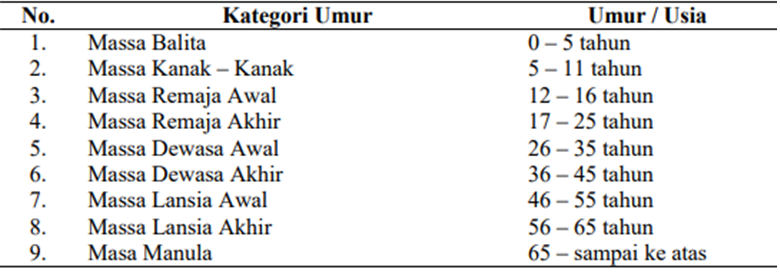
\includegraphics[scale=0.6]{gambar/umur.png}
    % Label referensi dari gambar yang diinputkan
    \label{fig:Umur}
\end{figure}

\begin{center}
    % Keterangan gambar yang diinputkan
    Gambar 2.1 : Kategori umur menurut Depkes. RI (2009)
\end{center}

\subsection{Gender}
Gender merupakan perbedaan yang terlihat antara laki-laki dan perempuan apabila dilihat dari penampilan 
dan tingkah laku. Gender dapat didefinisikan sebagai keadaan dimana individu yang lahir secara biologis 
sebagai laki-laki dan perempuan yang kemudian memperoleh pencirian sosial sebagai laki-laki dan perempuan 
melalui atribut maskulinitas dan feminimitas yang diperlihatkan individu tersebut\citep{LanguageGender}.

\subsection{Etnis}
Kata etnis mengacu pada suatu golongan atau kelompok manusia yang anggota - anggotanya mengidentifikasikan 
dirinya dengan sesamanya, biasanya berdasarkan garis keturunan dan adat yang dianggap sama. Identitas 
etnis ditandai oleh pengakuan dari orang lain akan ciri khas kelompok tersebut seperti kesamaan budaya, 
bahasa, agama, perilaku, dan ciri-ciri biologis\citep{Ethnicity}.
% input gambar
\begin{figure} [H] \centering
    % Nama dari file gambar yang diinputkan
    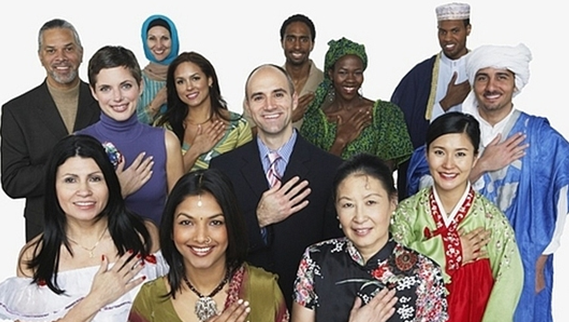
\includegraphics[scale=0.6]{gambar/etnik.png}
    % Label referensi dari gambar yang diinputkan
    \label{fig:Etnik}
\end{figure}

\begin{center}
    % Keterangan gambar yang diinputkan
    Gambar 2.2 : Macam-macam Etnik di dunia
\end{center}

\subsection{Visi Komputer}
Visi komputer adalah bidang ilmiah interdisipliner yang membahas bagaimana komputer dapat memperoleh 
pemahaman tingkat tinggi dari gambar atau video digital. Dari perspektif teknik, bidang ini berupaya 
mengotomatiskan tugas-tugas yang dapat dilakukan oleh sistem pengelihatan  manusia. Tugas  penglihatan 
komputer   meliputi metode untuk memperoleh, memproses, menganalisis dan memahami gambar digital, dan 
ekstraksi data dimensi tinggi dari dunia nyata untuk menghasilkan informasi numerik atau simbolis, 
misalnya dalam bentuk keputusan. Pengertian dalam konteks ini berarti transformasi gambar visual 
(input retina) menjadi deskripsi mengenai dunia sekitar yang dapat berinteraksi dengan proses pemikiran 
lain dan memperoleh tindakan yang sesuai. Pemahaman gambar ini dapat dilihat sebagai penguraian informasi 
simbolik dari data gambar menggunakan model yang dibangun dengan bantuan geometri, fisika, statistik, dan 
teori pembelajaran. Sub-domain dari pengelihatan komputer meliputi rekonstruksi adegan, deteksi peristiwa, 
pelacakan video, pengenalan objek, estimasi pose 3D, pembelajaran, pengindeksan, estimasi gerakan, dan 
pemulihan gambar\citep{MachineVisionMachineLearning}.

\subsection{Machine Learning}
\textit{Machine Learning (ML)} atau Pembelajaran Mesin merupakan bagian dari \textit{Artificial Intelligence (AI)} yang 
bertujuan untuk memberi optimalisasi dalam kriteria dengan cara menganalisa sampel data yang terdahulu 
yang sudah disimpan atau direkam untuk menghasilkan sebuah prediksi. Sehingga manusia tidak perlu 
mengindentifikasi sebuah proses sepenuhnya, karena dengan \textit{Machine Learning}, komputer mampu membuat pola 
untuk membuat keputusan. \textit{Machine Learning} melakukan \textit{training} yang merupakan proses pembelajaran terhadap 
model data yang sudah terdefinisikan ke beberapa parameter \textit{(data training)} yang menghasilkan beberapa 
pola sehingga komputer dapat melakukan proses klasifikasi berdasarkan pola atau ciri-ciri yang sudah 
didapatkan dalam proses \textit{training}. Kemudian komputer dapat memberikan sebuah prediksi pada data baru 
selanjutnya berdasarkan hasil training. \textit{Machine Learning} dapat memberi solusi dalam berbagai permasalahan
seperti \textit{Computer Vision} (Visi Komputer), \textit{Speech Recognition} (Pengenalan Suara) dan \textit{Robotics} (Robotika)\citep{MachineLearning}.

\subsection{Deep Learning}
\textit{Deep Learning} merupakan \textit{artificial neural network} yang memiliki banyak \textit{layer} dan \textit{synapse weight}. 
\textit{Deep learning} dapat menemukan relasi tersembunyi atau pola yang rumit antara \textit{input} dan \textit{output}, yang 
 tidak dapat diselesaikan menggunakan \textit{multilayer perceptron}. Keuntungan  utama  \textit{deep  learning}  yaitu 
 mampu merubah data dari \textit{nolinearly separable} menjadi \textit{linearly separable} melalui serangkaian transformasi 
 \textit{(hidden layers)}. Selain itu, \textit{deep learning} juga mampu mencari \textit{decision boundary} yang berbentuk \textit{non-linier}
 , serta mengsimulasikan interaksi \textit{non-linier} antar fitur. Jadi, input ditransformasikan secara 
 \textit{non-linier} sampai akhirnya pada output, berbentuk distribusi \textit{class-assignment}\citep{DeepLearning}.

 \begin{figure} [H] \centering
    % Nama dari file gambar yang diinputkan
    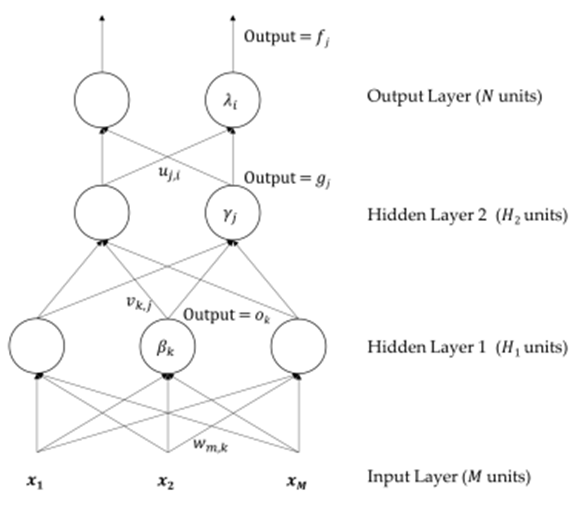
\includegraphics[scale=0.6]{gambar/deeplearning.png}
    % Label referensi dari gambar yang diinputkan
    \label{fig:Deep Learning}
\end{figure}

\begin{center}
    % Keterangan gambar yang diinputkan
    Gambar 2.3 : \textit{Deep Learning 4 layer}
\end{center}

\subsection{Convolutional Neural Network (CNN)}
\textit{Convolutional Neural Network (CNN)} merupakan cabang dari \textit{Multilayer Perceptron (MLP)} yang digunakan untuk
mengolah data dua dimensi. \textit{CNN} memiliki kedalaman jaringan yang tinggi sehingga \textit{CNN} termasuk dalam jenis
\textit{Deep Neural Network}. Perbedaan \textit{CNN} dengan \textit{MLP} terdapat pada neuron dimana pada \textit{MLP} setiap neuron hanya
berukuran satu dimensi, sedangkan \textit{CNN} setiap neuronnya berukuran dua dimensi. Pada \textit{CNN}, operasi linier
menggunakan operasi konvolusi\citep{CNN}.

\subsection{Image Processing}
\textit{Image Processing} atau Pengolahan Citra merupakan teknik dalam pemrosesan gambar dengan input berupa 
citra dua dimensi yang bertujuan untuk menyempurnakan citra atau mendapatkan informasi yang berguna 
untuk diolah menjadi beberapa keputusan. Dalam operasi pemrosesan citra, operasi yang sering dilakukan 
dalam format gambar \textit{grayscale}. Gambar \textit{grayscale} didapatkan dari pemrosesan gambar berwarna yang 
didekomposisi menjadi komponen merah (R), hijau (G) dan biru (B) yang diproses secara independen sebagai 
gambar \textit{grayscale}. Image Processing terbagi menjadi dalam tiga tingkatan\citep{ImageProcesing}:
    \begin{enumerate}
        \item \textit{Low-Level Image Processing} \\
        \textit{Low-Level Image Processing} merupakan operasi sederhana dalam pengolahan gambar dimana input dan 
        output berupa gambar. Contoh: \textit{contrast enchancement} dan \textit{noise reduction}.
        \item \textit{Mid-Level Image Processing} \\
        \textit{Mid-Level Image Processing} merupakan operasi pengolahan gambar yang melibatkan ekstrasi atribut dari 
        gambar input. Contoh: \textit{edges, contours} dan \textit{regions}.
        \item \textit{High-Level Image Processing} \\
        \textit{High-Level Image Processing} merupakan merupakan kategori yang melibatkan pemrosesan gambar kompleks 
        yang terkait dengan analisis dan interpretasi konten dalam sebuah keadaan untuk pengambilan keputusan.
    \end{enumerate}

\subsection{Digital Image}
\textit{Digital Image} merupakan fungsi dua dimensi f(x,y) yang merupakan proyeksi dari bentuk tiga dimensi kedalam 
bentuk dua dimensi dimana x dan y merupakan lokasi elemen gambar atau piksel yang berisikan nilai. Ketika
nilai x,y dan intensitasnya berupa diskrit, maka gambar tersebut dapat dikategorikan sebagai digital
image. Secara matematis, \textit{digital image} adalah representasi matriks dari gambar dua dimensi menggunakan
piksel. Setiap piksel  diwakili  oleh  nilai  numerik. Untuk  gambar  \textit{grayscale},  hanya  memiliki  
satu  nilai dengan kisaran antara 0-255.Pada Gambar 2.5, untuk gambar yang berwarna, memiliki tiga 
nilai yang mewakili merah (R), hijau (G) dan biru (B) yang masing-masing memiliki kisaran nilai yang 
sama antara 0-255. Jika suatu gambar hanya memiliki dua intensitas, gambar tersebut dikenal sebagai 
\textit{binary image}\citep{ImageProcesing}.
